\documentclass[doc,a4paper,man,natbib,floatsintext,noextraspace]{apa6}\usepackage[]{graphicx}\usepackage[]{color}
% maxwidth is the original width if it is less than linewidth
% otherwise use linewidth (to make sure the graphics do not exceed the margin)
\makeatletter
\def\maxwidth{ %
  \ifdim\Gin@nat@width>\linewidth
    \linewidth
  \else
    \Gin@nat@width
  \fi
}
\makeatother

\definecolor{fgcolor}{rgb}{0.345, 0.345, 0.345}
\newcommand{\hlnum}[1]{\textcolor[rgb]{0.686,0.059,0.569}{#1}}%
\newcommand{\hlstr}[1]{\textcolor[rgb]{0.192,0.494,0.8}{#1}}%
\newcommand{\hlcom}[1]{\textcolor[rgb]{0.678,0.584,0.686}{\textit{#1}}}%
\newcommand{\hlopt}[1]{\textcolor[rgb]{0,0,0}{#1}}%
\newcommand{\hlstd}[1]{\textcolor[rgb]{0.345,0.345,0.345}{#1}}%
\newcommand{\hlkwa}[1]{\textcolor[rgb]{0.161,0.373,0.58}{\textbf{#1}}}%
\newcommand{\hlkwb}[1]{\textcolor[rgb]{0.69,0.353,0.396}{#1}}%
\newcommand{\hlkwc}[1]{\textcolor[rgb]{0.333,0.667,0.333}{#1}}%
\newcommand{\hlkwd}[1]{\textcolor[rgb]{0.737,0.353,0.396}{\textbf{#1}}}%
\let\hlipl\hlkwb

\usepackage{framed}
\makeatletter
\newenvironment{kframe}{%
 \def\at@end@of@kframe{}%
 \ifinner\ifhmode%
  \def\at@end@of@kframe{\end{minipage}}%
  \begin{minipage}{\columnwidth}%
 \fi\fi%
 \def\FrameCommand##1{\hskip\@totalleftmargin \hskip-\fboxsep
 \colorbox{shadecolor}{##1}\hskip-\fboxsep
     % There is no \\@totalrightmargin, so:
     \hskip-\linewidth \hskip-\@totalleftmargin \hskip\columnwidth}%
 \MakeFramed {\advance\hsize-\width
   \@totalleftmargin\z@ \linewidth\hsize
   \@setminipage}}%
 {\par\unskip\endMakeFramed%
 \at@end@of@kframe}
\makeatother

\definecolor{shadecolor}{rgb}{.97, .97, .97}
\definecolor{messagecolor}{rgb}{0, 0, 0}
\definecolor{warningcolor}{rgb}{1, 0, 1}
\definecolor{errorcolor}{rgb}{1, 0, 0}
\newenvironment{knitrout}{}{} % an empty environment to be redefined in TeX

\usepackage{alltt}




\usepackage[english]{babel}
\usepackage[utf8x]{inputenc}
\usepackage{amsmath}
\usepackage{amsthm}
\usepackage{graphicx}
\usepackage[colorinlistoftodos]{todonotes}
\usepackage[singlespacing]{setspace}


\title{The Role of Shallow Processing in Agreement Attraction}
\shorttitle{Your APA6-Style Manuscript}
\author{Utku Türk, Pavel Loga\v{c}ev}
\affiliation{Boğaziçi University}


\abstract{We report the results of two speeded acceptability judgment experiments in Turkish. We hypothesized an alternative explanation for agreement attraction effects in Turkish that is based on shallow processing. Our findings contradict our hypothesized form-driven processing strategy and support an account of agreement attraction based on the use of abstract linguistic features, rather than mere form.}

\let\B\relax %to resolve a conflict in the definition of these commands between xyling and xunicode (the latter called by fontspec, called by charis)

\let\T\relax

\usepackage{xyling} %for trees; the use of xyling with the CharisSIL font produces poor results in the branches. This problem does not arise with the packages qtree or forest.
\usepackage[linguistics,edges]{forest} %for nice trees!
  
%\usepackage[block]{leipzig}
% input glosses
%\makeglossaries

%\newleipzig{aor}{aor}{aorist}

\usepackage{linguex}
\usepackage{hyperref}
\IfFileExists{upquote.sty}{\usepackage{upquote}}{}
\begin{document}

\maketitle


\section{Introduction} \label{sec:Intro}

% %\footnote{\printglossaries}. % add this to somewhere in the first page I suppose
% 
% \subsection{Agreement Attraction Thingy} \label{sec:Intro:literature}
% 
% \subsubsection{Morphophonology} \label{sec:Intro:literature:morphophonology}
% 
% %fill here accordingly to your results AFTER YOU WRITE THE RESULT.
% 
% 
% \subsubsection{related sub-sub-field studies} \label{sec:Intro:literature:others}
% 
% \subsubsection{This work details} \label{sec:Intro:literature:thiswork}

% \citet{LagoEtAl:2018} hypothesize that genitive NPs can trigger agreement attraction in Turkish, because Turkish makes heavy use of genitive subjects, which means genitives are a priori likely to function as agreement controllers. The underlying assumption is that agreement processes rely on, at least partially, the case of an NP to determine its fit for the role of an agreement controller. 
% If that is so, their items are problematic %as in ... give an example
% in that the marking on the head noun is ambiguous between possessive and accusative case, while only possessive-marked NPs qualify as agreement controllers. Therefore, if engaged in shallow processing, readers may be more likely to misidentify the genitive NP as the agreement controller when the head noun, which is the only other alternative, is ambiguous, compared to when it is not.

% In Experiment 1, we decided to test this hypothesis 




\section{Experiment 1} \label{sec:exp1}

% do not do this in one chunk. differentiate the chunks and give them proper names.


In Experiment 1, we tested whether speakers of Turkish make fewer agreement attraction errors when the local ambiguity in the head noun is resolved. 
Specifically, we tried to replicate \citet{LagoEtAl:2018} study. However, instead of using morphologically ambiguous head nouns, we uses nouns ending in a vowel, thus resolving the ambiguity between the accusative and possessive. 

\subsection{Participants} \label{sec:exp1:participants}

We recruited 118 undergraduate students to participate in Experiment 1 in exchange for course credit. All participants were native speakers of Turkish, with an average age of 20 (range: 18 -- 32). 
These items were not included in the analysis. Experiments in this paper were carried out following the Declaration of Helsinki and the regulations concerning ethics at research in Bo\u{g}azi\c{c}i University. All participants provided informed consent. They were tested online, on IbexFarm. 
%to-do: cite ibexfarm

\subsection{Materials} \label{sec:exp1:materials}

We used 40 sets of sentences like (\ref{item:exp1ExperimentalItems}), in which we manipulated 
(i) the number of the attractor noun, and
(ii) the number agreement on the verb. 
Plural number and plural agreement were both marked with the affix \textit{-ler/-lar}, while singular number and singular agreement were marked with its absence. 
%
All sentences started with a complex subject NP like \textit{`the manager's cook'} (\textit{yöneticinin aşcısı}), in which the possessor, which functioned as the attractor, carried genitive case, and the head noun cassied possessive case. Because the head noun was singular in all conditions, sentences with plural verb agreement were ungrammatical.
% to-do: Didn't we use Lago's items as a base?? If so, we need to say this here, and also how much we've changed, and how much remained.
Unlike the \citet{LagoEtAl:2018} sentences, our head nouns were vowel-ending, and therefore not ambiguous between accusative case, for which the case suffix is \textit{-yI}, and possessive case, for which the suffix is \textit{-sI}. 

% to-do: This all needs to go up, to the description of the potential confound in Lago et al.'s study.
%This change was due to the morpho-phonologic nature of possessive suffix in Turkish, which spell-outs as (\textit{-I}) after a consonant same as the accusative. 
The distribution of the verb types followed the same pattern as in \citet{LagoEtAl:2018}, namely twenty unergatives, eighteen unaccusatives, and two optionally transitive verbs. 
%
The pre-verbal adverbials preceding the verb in our experimental sentences consisted of 2-3 words (15 characters on average). 

% to-do: Why are all sentences in aorist instead of past (as they are in the actual items)?
\ex. \label{item:exp1ExperimentalItems}
%
\a. \textsc{Plural Attractor, Ungrammatical (Plural Verb)} \label{item:exp1expitem-plpl}\\ 
  \gll *[Yönetici-ler-in \textbf{aşcı-sı}] mutfak-ta sürekli \textbf{zıpl-ıyor-lar}.\\ 
  manager-\textsc{pl}-\textsc{gen}  cook-\textsc{poss} kitchen-\textsc{loc} non-stop  jump-\textsc{prog}-\textsc{pl}.\\
  \glt \textit{`The cooks of the manager were jumping in the kitchen non-stop.'}
%
\b. \textsc{Plural Attractor, Grammatical (Singular Verb)} \label{item:exp1expitem-plsg}\\ 
  \gll [Yönetici-ler-in \textbf{aşcı-sı}] mutfak-ta sürekli \textbf{zıpl-ıyor}.\\ 
  manager-\textsc{pl}-\textsc{gen}  cook-\textsc{poss} kitchen-\textsc{loc} non-stop  jump-\textsc{prog}.\\
  \glt \textit{`The cooks of the manager was jumping in the kitchen non-stop.'}
%
\c. \textsc{Singular Attractor, Ungrammatical (Plural Verb)} \label{item:exp1expitem-sgpl}\\ 
  \gll *[Yönetici-nin \textbf{aşcı-sı}] mutfak-ta sürekli \textbf{zıpl-ıyor-lar}.\\ 
  manager-\textsc{gen}  cook-\textsc{poss} kitchen-\textsc{loc} non-stop  jump-\textsc{prog}-\textsc{pl}.\\
  \glt \textit{`The cook of the manager were jumping in the kitchen non-stop.'}
%
\d. \textsc{Singular Attractor, Grammatical (Singular Verb)}\label{item:exp1expitem-sgsg}\\ 
  \gll [Yönetici-nin \textbf{aşcı-sı}] mutfak-ta sürekli \textbf{zıpl-ıyor}. \\ 
  manager-\textsc{gen}  cook-\textsc{poss} kitchen-\textsc{loc} non-stop  jump-\textsc{prog}.\\
  \glt \textit{`The cook of the manager was jumping in the kitchen non-stop.'}

We intermixed our experimental sentences with 40 filler sentences of two types, as illustrated in (\ref{item:exp1FillerItems}). To compensate for the fact that among experimental sentences, all ungrammatical sentences ended in a plural-agreeing verb, while all grammatical sentences ended in a singular-agreeing verb, we included 20 grammatical sentences with plural verbs, and 20 ungrammatical sentences with singular agreement. This was done in order to discourage participants from using a strategy based on verb number. 

%Even though filler items did not follow a strict template as the experimental items, they were created within a template of \textit{Noun$_{{\textsc{gen}}}$-Noun$_{{\textsc{gen}}}$-Converb-Noun-Adverb-Verb}. The ungrammaticality was created non-locally in the filler items to avoid task strategies. Example filler sentences can be seen in \ref{item:exp1FillerItems}.


\ex. \label{item:exp1FillerItems}
%
\a. \textsc{Grammatical Filler (Plural Verb)}\\ 
  \gll [Sosyolog-un \textbf{öğrenci-si}] konuş-unca tutarsızlık açığ-a \textbf{çıkar-dı-lar}.\\ 
  sociolog-\textsc{gen}  student-\textsc{poss} speak-\textsc{nmlz} inconsistency  open-\textsc{dat} deduct-\textsc{pst}-\textsc{pl}.\\
  \glt \textit{`When the sociologist's student talked, they exposed an inconsistency.'}
%to-do: Translation above doesn't make sense.
%
%
\b. \textsc{Ungrammatical Filler (Singular Verb)}\\ 
\gll *[Dansöz-ün \textbf{koca-sı}] var-ınca kapı sakince \textbf{aç-tı}.\\ 
dancer-\textsc{gen}  husband-\textsc{poss} arrive-\textsc{nmlz} door slowly  open-\textsc{pst}.\\
\glt \textit{Intended:`When the husband of the dancer came, the door opened slowly.'}
% to-do: Does the above mean that it's grammatical with another meaning?

\subsection{Procedure} \label{sec:exp1:procedure}

The experiment was run online, using the web-based platform Ibex Farm (\url{http://spellout.net/ibexfarm/}). Each experimental session took approximately XXX minutes to complete.
% to-do: How much time did it take?
%
Prior to the start of the experiment, participants provided demographic information, as well as informed consent to participate in the experiment. They read the instructions, and were given 9 practice trials before the experiment began.
%
Each trial began with a blank screen for 600 ms, followed by a word-by-word RSVP presentation of the sentence in the center of the screen, followed by an acceptability judgment. 
Sentences were presented word-by-word in 30pt font size, and at a rate of 400 ms per word. Participants pressed the key 'P' for \textit{'acceptable'} and 'Q' for \textit{'unacceptable'}. They were instructed to provide an acceptability rating before the 5,000 ms deadline. During the experiment, they were reminded to respond faster if they responded too slowly. 

Participants saw 40 experimental and 40 filler sentences. Experimental sentences were distributed among four different lists according to a Latin-square design. Every participant saw one version of the experiment with a specific list and one item per condition.   

\subsection{Analysis} \label{sec:exp1:analysis}

Since our aim was to test whether the morphological ambiguity present in the \citet{LagoEtAl:2018} items affected the presence or magnitude of the agreement attraction effect, statistically, we needed to test for the presence of an interaction between (i) the presence of the morphological ambiguity on the head noun, and (ii) the agreement attraction effect. In order to do so, we decided to analyze the data from the present experiment together with Lago et al.'s data, using experiment as an additional factor in the analysis.

%All experimental trials from both experiments (Experiment 1 and Lago et al.'s study) was included in the analysis. 

Prior to analysis we removed the data for all participants who failed to show sufficient sentitivity to the effect of grammaticality in singular attractor conditions, i.e., when no agreement attraction was expected. Specifically, we removed all participants for whom the difference in the percentage of `yes' responses between the grammatical condition \ref{item:exp1expitem-sgsg} and the ungrammatical condition \ref{item:exp1expitem-sgpl} was below the threshold of 25 percentage points. As a result, we excluded 10 participants from experiment 1, and  one participant from the Lago et al. experiment.

We used the R packages brms \citep{R-brms_b} and rstan \citep{R-stan} to fit Bayesian hierarchical models \citep[e.g.,]{GelmanHill:2007}. We analyzed only experimental sentences, and used (i) grammaticality of the sentence, (ii) attractor number, and (iii) presence of morphological ambiguity (i.e., experiment), as well as all their interactions as predictors. Moreover, we used by-participant and by-item intercepts and slopes for all predictors.

Data for experiment 1, along with our analysis scripts can be found \texttt{link hidden due to blind review}.
% to-do: Please create a repo where we can put all of this, or specify the github URL. I'm not aware of any blind reviews.


\subsection{Results} \label{sec:exp1:results}






\autoref{fig:exp1AvgResponse} shows the average proportions of ‘acceptable’ responses by experimental condition for both the original experiment in \citet{LagoEtAl:2018} and our replication with unambiguous possessive marking. 
%
It shows that ungrammatical sentences with plural attractors are rated as acceptable more often
(M = 0.22, 
SE = 0.01) 
than their counterparts with singular attractors 
(M=0.11, 
SE=0.01).
%
%
%This means that ungrammatical sentences with plural attractors were classified as acceptable more often than their counterparts with singular attractors. 
The magnitude of the effect (0.10) was in line with the findings reported in \citet{LagoEtAl:2018}, where the difference was 0.11.
%
Accuracy rates for grammatical conditions were nearly equal
%
(M = 0.93 and 0.92, SE = 0.01 and 0.01, for singular and plural attractors respectively). 


\begin{knitrout}
\definecolor{shadecolor}{rgb}{0.969, 0.969, 0.969}\color{fgcolor}\begin{figure}

{\centering 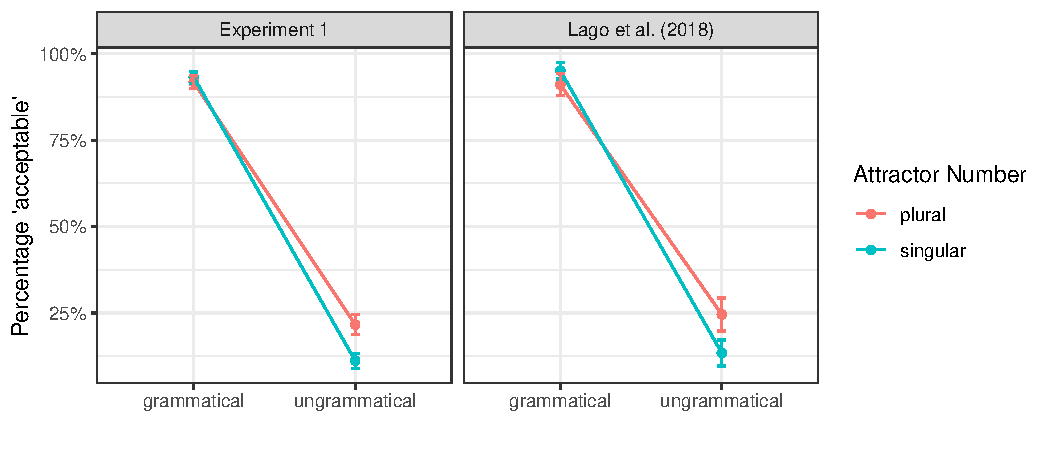
\includegraphics[width=\maxwidth]{figure/exp1AvgResponse-1} 

}

\caption{Average percentages of `acceptable' responses in Experiment 1 and \citet{LagoEtAl:2018}. Within-subject 95\% confidence intervals in brackets \cite{Cousineau:2005,Morey:2008}.}\label{fig:exp1AvgResponse}
\end{figure}


\end{knitrout}



A Bayesian GLM assuming a Bernoulli distribution with a probit-link function was fit to participants' `acceptable' responses. The model's estimates and 95\% credible intervals are shown in \autoref{fig:exp1ResponseModel}. 
%
%They confirm the observations we stated above: the positive interaction between sentence grammaticality and attractor number is in line with a larger effect of attractor number in ungrammatical sentences. 
%
The main effect of \textit{ungrammaticality} ($\hat{\beta}=-3.09;$ $CI=[-3.35; -2.84];$ $P(\beta<0)> .999$) indicates that, on average, participants were quite good at distinguishing between grammatical and ungrammatical sentences. Meanwhile, the positive interaction between \textit{ungrammaticality} and \textit{attractor number} ($\hat{\beta}=0.72;$ $CI=[0.42; 1.02];$ $P(\beta<0)< .001$) indicated a larger effect of attractor number in ungrammatical conditions, and thus a number agreement attraction effect.
Importantly, there was no evidence for a three-way interaction between \textit{the presence of ambiguity}, \textit{ungrammaticality} and \textit{attractor number} ($\hat{\beta}=0.30;$ $CI=[-0.20; 0.79];$ $P(\beta<0)=    .12$).

% to-do:
% Importantly, even if there was an interaction with experiment, it's relatively small, so it wouldn't reduce the other interaction to 0. 

%Moreover, this findings are also predicted by cue-based retrieval models \citep{engelmann2019effect, vasishth2019computational} and last rendition of marking and morphing theory by \citet{HammerlyEtAl:2019}. %does it tho? especially with regards to what sol lago says: gen and morphophonology gives clues. maybe we should take a look at speeded acceptability? 
%maybe this is not the perfect place to write this.


\begin{knitrout}
\definecolor{shadecolor}{rgb}{0.969, 0.969, 0.969}\color{fgcolor}\begin{figure}

{\centering 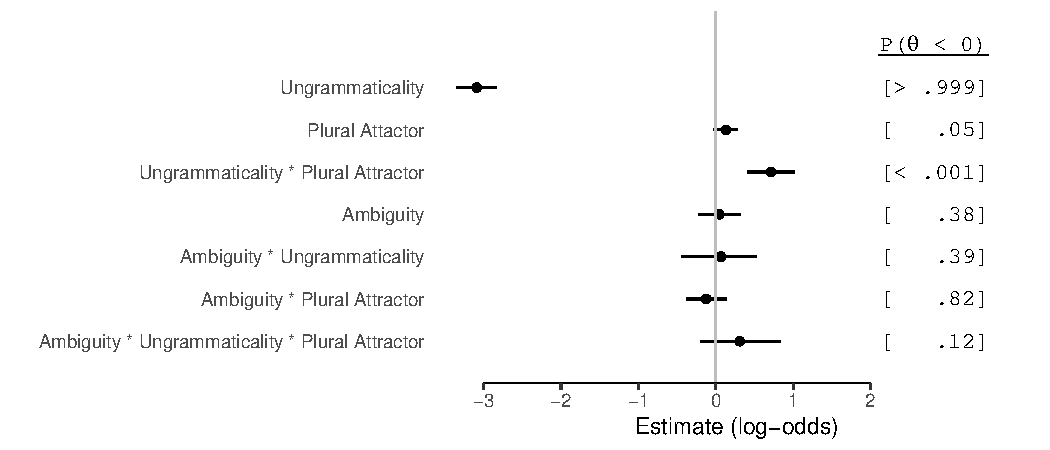
\includegraphics[width=\maxwidth]{figure/exp1ResponseModel-1} 

}

\caption[Estimates and 95\% credible intervals for the regression coefficients for Experiment 1]{Estimates and 95\% credible intervals for the regression coefficients for Experiment 1.}\label{fig:exp1ResponseModel}
\end{figure}


\end{knitrout}



\subsection{Discussion} \label{sec:exp1:discussion}

In Experiment 1, we have found number attraction effects in Turkish using genitive possessive structures, as it is also attested in \citet{LagoEtAl:2018}. To account for their findings, \citet{LagoEtAl:2018} assume a cue-based memory retrieval mechanism. That is, they assume that upon reaching the verb, the parser attempts to retrieve its agreement controller (the subject) using a cue-based retrieval mechanism \citep{LewisVasishth:2005,JagerEngelmannVasishth:2017}. The assumption is that in sentences such as \ref{item:exp1ExperimentalItems}, features such as case and number information are used to identify the agreement controller in memory. In ungrammatical sentences, when the verb bears plural agreement, no NP in memory will match both retrieval cues. However, in ungrammatical plural attractor conditions, the attractor matches one of the cues, which can lead to its erroneous retrieval on some occasions. This cannot happen in ungrammatical singular attractor conditions. This difference in the probability of erroneous retrievals is presumably what surfaced as a number agreement attraction effect, as observed in \citet{LagoEtAl:2018}, and our Experiment 1.

In their work, \citet{LagoEtAl:2018} argue that the agreement attraction in genitive-possessive structures in Turkish is due to the use of genitive case as a marker of embedded subjects in Turkish, i.e. differential subject marking (DSM) properties of Turkish \citep{kornfilt2009dom}. They argue that the genitive case in Turkish may not provide strong cue against subjecthood due to DSM while it does in English. Following this logic, we hypothesized that the other phenomenon that gives a strong clue against the subject should inhibit the illusionary dependencies as argued in \citet{nicol2016minimal}. One such phenomenon was present in the experimental items used in \citet{LagoEtAl:2018}: the morpho-phonologic ambiguity between the accusative and the possessive case. Since they use only consonant ending heads, the marking on the head is ambiguous between the accusative and the possessive marking. Following their argumentation, participants may search for other agreement controllers than the possessive marked heads when they are engaged in shallow processing and erroneously assign head as genitive marked distractor.

Nevertheless, we found that when the possessive marker is disambiguated agreement attraction does not diminish in effect size. As seen in \autoref{fig:exp1ResponseModel}, we successfully replicated the findings of \citet{LagoEtAl:2018} with disambiguated head nouns. Thus, we conclude that the morpho-phonological possessive-accusative ambiguity plays no role in number attraction in Turkish.


However, there is an alternative explanation that has yet to be ruled out: task-specific strategies. We hypothesized that readers may engage in an even shallower process in the evaluation of the sentences such as \ref{item:exp2ExperimentalItems} in which readers decide on the acceptability of the sentence with a faulty state of memory. In our model, we claim that after they read the sentence readers may end up with insufficient information to reliably judge the sentence. Upon such cases, readers may end up using extremely shallow processing methods such as matching the agreement-wise unrelated but form-wise related elements. % I should try a bit more to explain this part, I did not do a good job here.
We present our hypothesized decision tree in \autoref{fig:mptModel}

\begin{figure}[h]
    \centering
                      \begin{forest}
                  for tree = {
                  % nodes
                      draw, 
                      align=center,
                      minimum height=5ex,
                      minimum width=3em,
                      font=\linespread{0.84}\selectfont,
                  % tree
                      grow'=0,
                      parent anchor=east,
                      child  anchor=west,
                      s sep = 4mm,    
                      l sep = 12mm, 
                  % edge
                      edge = {semithick},
                  % level styles
                  if level = 0{}{rounded corners=2ex},
                  where n children=0{tier=level, sharp corners}{calign=edge midpoint},
                  % edge labels
                  EL/.style={edge label={node [pos=0.5, fill=white,
                                               font=\scriptsize\sffamily,
                                               inner sep=2pt] {$#1$}}
                                      }
                              }% end for tree
                  [,coordinate
                  [target\\ item,no edge
                      [recolection\\ certainity, EL=r
                          ["yes"]
                      ]
                      [recolection\\ uncertainity, EL=1-r,
                          [guess "yes", tier=L1, EL=g,
                              ["yes"]
                          ]
                          [guess "no", tier=L1, EL=1-g
                              ["no"]
                          ]
                      ]
                  ]
                  [,coordinate, no edge]
                  [target\\ item, no edge
                      [guess "yes", tier=L1, EL=g,
                              ["yes"]
                      ]
                      [guess "no", tier=L1, EL=1-g
                          ["no"]
                      ]
                   ]
                  ]
                      \end{forest} 
    \caption{Proposed multinomial processing tree of how people judge sentences in an agreement attraction task}
    \label{fig:mptModel}
\end{figure}

The aim of our second experiment was to test whether agreement attraction in Turkish may be an instance of a \textit{form-driven processing strategy}. Assuming that readers sometimes engage in shallow processing, they may end up with insufficient information to reliably classify a sentence as (un)acceptable. In such cases, participants may choose to classify sentences with plural-agreement-bearing verbs as acceptable if they have a memory of a nominal plural morpheme in the sentence. Such a response strategy would lead to a larger number of ‘acceptable’ responses in ungrammatical plural attractor conditions than in ungrammatical singular attractor conditions. 



\section{Experiment 2} \label{sec:exp2}







In Experiment 2, we wanted to rule out the possibility of \textit{form-driven processing strategy}, namely participants deciding on the acceptability of a sentence using a memory of plural morpheme in the sentence when they do not have sufficient information to rate sentences (un)acceptable. 
 

\subsection{Participants} \label{sec:exp2:participants}

We recruited 79 native speakers of Turkish to participate in Experiment 2. Their average age was 21, ranging from 18 to 31. 


Experiments in this paper were carried out following the Declaration of Helsinki and the regulations concerning ethics in research in Bo\u{g}azi\c{c}i University. All participants provided informed consent. They were tested online, on IbexFarm, using their preferred platform, % Find citation for using IbexFarm and online testing etc?


\subsection{Materials} \label{sec:exp2:materials}

In Experiment 2, participants saw the sentences word by word in the middle of their screen. We have again formed 40 sets of items. The grammaticality of the sentences (\textit{grammatical} x \textit{ungrammatical}) and the number of the attractor (\textit{singular} x \textit{plural}) were manipulated. Unlike Experiment 1, we used nominalized relative clause attractors instead of nouns. We took advantage of syncretism between Turkish nominal and verbal plural marker. Both of these morphemes spells-out as \textit{-lAr}, which enables us to check whether agreement attraction in Turkish can be explained by an extremely shallow dependency parsing based on the forms of morphemes rather than linguistic features.

All experimental sentences followed the same template as the experiment one except for the nature of the attractor: \textit{RC-Bare Noun-Adverb-Verb}. 
We have used the same verbs, and have not changed the distribution of verb types. We also utilized the same or extremely similar adverbials in length. We again did not manipulate the number of the head noun and manipulated the number of the attractor. Relative clauses we used in this experiment are all object relative clauses and they are all marked with canonical \textit{-dIK} nominalizer. Since Turkish is a pro-drop language, we also dropped the subject within the embedded clause, thus ending up with a one-word object relative clause whose head is also the controller of the number agreement on the matrix verb. One example set of experimental items can be seen in \ref{item:exp2ExperimentalItems}.


\ex. \label{item:exp2ExperimentalItems}
%
\a. \textsc{Plural Attractor, Ungrammatical (Plural Verb)}\label{item:exp2expitem-plpl}\\ 
  \gll *Tut-tuk-lar-ı aşcı mutfak-ta sürekli zıpl-ıyor-lar.\\ 
  hire-\textsc{nmlz}-\textsc{pl}-\textsc{poss}  cook kitchen-\textsc{loc} non-stop  jump-\textsc{prog}-\textsc{pl}.\\
  \glt \textit{`The cook that they hired were jumping in the kitchen non-stop.'}
%
\b. \textit{Plural Attractor, Grammatical (Singular Verb)}\label{item:exp2expitem-plsg}\\ 
  \gll Tut-tuk-lar-ı aşcı mutfak-ta sürekli zıpl-ıyor.\\ 
  hire-\textsc{nmlz}-\textsc{pl}-\textsc{poss}  cook kitchen-\textsc{loc} non-stop  jump-\textsc{prog}.\\
  \glt \textit{`The cook that they hired was jumping in the kitchen non-stop.'}
%
\c. \textit{Singular Attractor, Ungrammatical (Plural Verb)}\label{item:exp2expitem-sgpl}\\
  \gll *Tut-tuğ-u aşcı mutfak-ta sürekli zıpl-ıyor-lar.\\ 
  hıre-\textsc{nmlz}-\textsc{poss}  cook kitchen-\textsc{loc} non-stop  jump-\textsc{prog}-\textsc{pl}.\\
  \glt \textit{`The cook that they hired were jumping in the kitchen non-stop.'}
%
\d. \textit{Singular Attractor, Grammatical (Singular Verb)}\label{item:exp2expitem-sgsg}\\ 
  \gll Tut-tuğ-u aşcı mutfak-ta sürekli zıpl-ıyor.\\ 
  hıre-\textsc{nmlz}-\textsc{poss}  cook kitchen-\textsc{loc} non-stop  jump-\textsc{prog}.\\
  \glt \textit{`The cook that they hired was jumping in the kitchen non-stop.'}

In our filler items for Experiment 2, we made sure that every sentence starts with an object relative clause. We used plural distractors with grammatical verbs and singular distractors with ungrammatical verbs. In all of our filler sentences, the dependency between the first NP subject and its verb resolved in an adverbial embedded sentence. Grammatical filler items in Experiment 2 all had a template of
XXX
%\textit{RC$_{\textsc{pl}}$-Bare Noun-Adverb-Converb-Noun-Adverb-Verb$_{\textsc{pl}}$}, 
whereas ungrammatical filler items used a template of 
XXX
%\textit{RC$_{\textsc{sg}}$-Bare Noun-Adverb-Converb-Noun-Adverb-Verb$_{\textsc{sg}$}

Again, to avoid a possible strategy where participants use plural ending as a direct indication of ungrammaticality, half of our fillers were with an overt plural marking on a grammatical verb while the other half were without an overt plural marking on an ungrammatical verb. We used Turkish pro-drop characteristics which enable participants to form a dependency between the matrix verb and the null subject. Example filler sentences can be seen in \ref{item:exp2FillerItems} 

\ex. \label{item:exp2FillerItems}
%
\a. \textit{Plural Grammatical Verb}\\ 
  \gll Oku-t-tuk-lar-ı öğrenci başarılı ol-unca mutlu ol-du-lar.\\ 
  read-\textsc{caus}-\textsc{nmlz}-\textsc{pl}-\textsc{poss}  student successful be-\textsc{nmlz} happy be-\textsc{pst}-\textsc{pl}.\\
  \glt `When the student they sponsored become successful, they became happy.' 
%
\b. \textit{Singular Ungrammatical Verb}\\ 
  \gll *Kandır-dığ-ı adam öde-me-yince bulaşık saatlerce yıka-dı.\\ 
  trick-\textsc{nmlz}-\textsc{poss}  man pay-\textsc{neg}-\textsc{nmlz} dish for.hours clean-\textsc{pst}.\\
  \glt Intended:`When the man he tricked did not pay, he cleaned dishes for hours.'


\subsection{Procedure and Analysis} \label{sec:exp2:procedure_analysis}





% to-do: some more details.
% In Experiment 2, the same procedure as Experiment 1 has been followed with regards to how sentences are presented within the experiment. 

We analyzed the percentages of 'yes' answers given by the participants in experimental conditions. In the analysis of this experiment, we have included experimental items from our Experiments 1 and 2 to check the interaction between experiments and quantify the difference between verbal and nominal plural markers. In Experiment 2 as well, we excluded participants (1) who had more than 0.25 points of difference in accuracy between grammatical conditions, which implicates that they did not give enough attention to all conditions. We used R packages brms \citep{R-brms_b} and rstan \citep{R-stan} to fit Bayesian hierarchical models \citep{GelmanHill:2007}. We added our independent variables, i.e. grammaticality of the sentence and the overt number information on the distractors, and random variable experiment as a factor. Analyses by items and participants are also conducted as a 
part of the Bayesian hierarchical models. Data regarding our experiments and analysis can be found in \texttt{link hidden due to blind review}.

Across participants, a total 55 items were not responded to before the 5 second deadline by 45 different participants. These items were not included in the analysis. 

% Should I rephrase these parts?
%Prior the experiments, participant gave information regarding themselves and a consent to start to the experiment. They read the instructions where we showed what they will see in the experiment, what will be going to ask to participants, and where we informed them to be fast and accurate during the experiment. Every session started with practice session where participants have been informed being a bit faster when they were not. The sentences were presented in the middle of the screen word-by-word on a web-based platform Ibex Farm (\url{http://spellout.net/ibexfarm/}). Each word stayed on the screen for 300 ms, unlike \citet{LagoEtAl:2018} and \citet{WagersEtAl:2009} where words stayed for 500 ms in the screen. After the sentence is completed, participants were asked "How did they find the sentence?" They were informed to press P on their keyboard for \textit{good} and Q for bad. Apart from the practice items, we did not provide any feedback regarding their answer. However, participants were asked to be faster when they waited more than 5000 ms to answer the acceptability question.

\subsection{Results} \label{sec:exp2:results}

\autoref{fig:exp2AvgResponse} shows the average proportions of 'acceptable' responses by experimental conditions for both Experiment 1 and Experiment 2. We see that there is no effect resembling agreement attraction in the ungrammatical conditions of Experiment 2. Ungrammatical conditions showed comparable effects (0.05 and 0.06 for plural and singular attractors respeectively) regardless of the attractor's number.  

\begin{knitrout}
\definecolor{shadecolor}{rgb}{0.969, 0.969, 0.969}\color{fgcolor}\begin{figure}

{\centering 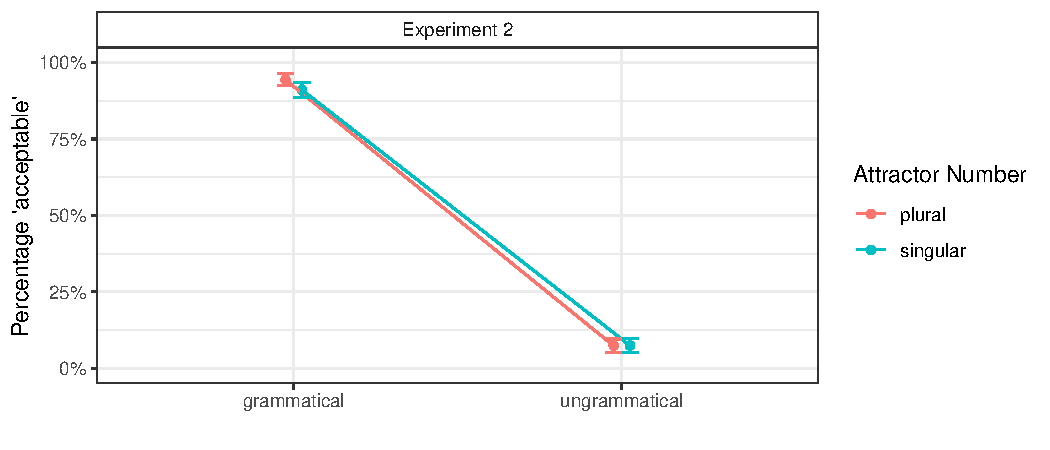
\includegraphics[width=\maxwidth]{figure/exp2AvgResponse-1} 

}

\caption{Estimates and 95\% credible intervals for the regression coefficients for Experiment 1 and Experiment 2.  Within-subject 95\% confidence intervals in brackets \cite{Cousineau:2005,Morey:2008}.}\label{fig:exp2AvgResponse}
\end{figure}


\end{knitrout}

The observations we made through \autoref{fig:exp2AvgResponse} also surfaces when we look at the estimates and 95\% CIs of a Bayesian GLM in \autoref{fig:exp2ResponseModel}. As is visible from the figure, the model shows a negative three-way interaction between grammaticality, type of attractor (nominal vs. verbal), and attractor number, which entails a reduced effect of agreement attraction in Experiment 2 compared to Experiment 1. 




\begin{knitrout}
\definecolor{shadecolor}{rgb}{0.969, 0.969, 0.969}\color{fgcolor}\begin{figure}

{\centering 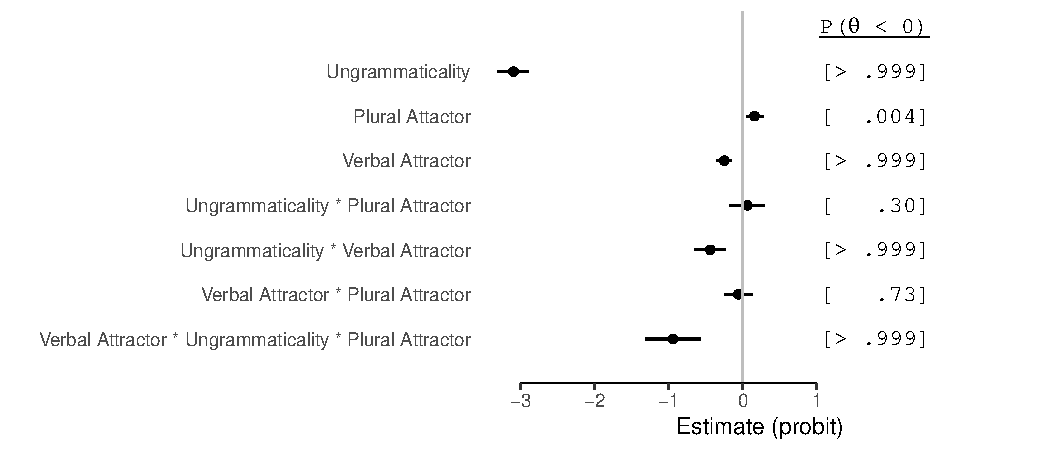
\includegraphics[width=\maxwidth]{figure/exp2ResponseModel-1} 

}

\caption[Estimates and 95\% credible intervals for the regression coefficients for Experiment 2]{Estimates and 95\% credible intervals for the regression coefficients for Experiment 2}\label{fig:exp2ResponseModel}
\end{figure}


\end{knitrout}


\subsection{Discussion} \label{sec:exp2:discussion}


In Experiment 2, we could not find any effect of agreement attraction in the acceptability ratings of ungrammatical conditions with a verbal plural attractor. However, number agreement attractions were observed when the attractors were nominal. Even though the forms of the two plural morphemes are the same form-wise, there is a distinct difference between the results of two experiments. One of the indications of zero-effect with verbal plural morpheme is that readers do not make decisions solely based on the form of the elements. This finding contradicts our hypothesized form-driven processing strategy and supports an account of agreement attraction based on the use of abstract linguistic features, rather than mere form.

However, results may be more telling with regards to the other theories of agreement attraction. These results seem unexpected within the cue-based retrieval mechanisms. Even though the root of the attractor is verbal, the morpheme is the same with the third person plural possessive marker since the relative clauses in Turkish are always nominalized and the subject is marked with the genitive case. The findings of this experiment indicate towards more fine-grained features needs to be utilized. One other possible explanation within the cue-based retrieval models can be formed around the status of agreement markers. One can say that the agreement process is completed in the verbal \textit{-lAr}; in other words, it is not the triggering morpheme but the probe of the agreement. This difference would mean that verbal \textit{-lAr} should not start any search for dependency resolution. In contrast to verbal \textit{-lAr}, the plural morpheme on the genitive is supposed to be triggering part of the agreement, not the probe. However, in Turkish embedded clauses, where genitive subjects can be seen, the number agreement works differently than the matrix level agreement. When the genitive subject of an embedded clause is marked with plural it is ungrammatical to have plural marking on the verb. 
This prohibition in return means that the genitive subjects should not create an expectation for a plural marked verb, which was believed to be the reason for the agreement attraction in \citet{LagoEtAl:2018}.


As for the marking and morphing theories, the results of Experiment 2 are completely expected and mitigated by the syntactic depth effects. Due to the genitive possessor's limited inner complexity compared to that of relative clause modifiers, marking and morphing theories would expect higher contribution from the genitive attractors to the final representation of number information. 


\section{General Discussion} \label{sec:general_discussion}



\bibliography{new-references,library}

\end{document}

%
% Please see the package documentation for more information
% on the APA6 document class:
%
% http://www.ctan.org/pkg/apa6
%
